\documentclass{article}
% \usepackage[czech]{babel}
% \usepackage[IL2]{fontenc}

\pagestyle{empty}
\usepackage[createtips]{fancytooltips}

\usepackage{fancybox}
\parindent 0 pt

\usepackage{color}
\definecolor{gray}{rgb}{0.8, 0.8, 0.8}
\definecolor{lightblue}{rgb}{0.7, 0.7, 1}
\definecolor{lightgreen}{rgb}{0.7, 1, 0.7}

\usepackage{multido,graphicx}
\usepackage[papersize={5in,5in},margin=1pt]{geometry}
\long\def\stranka#1#2{
\setbox0=\hbox{\begin{minipage}{2in}
\fboxsep 0 pt
\color{red}
\shadowbox{{\fboxsep 4pt\colorbox{yellow}
    {\begin{minipage}{\linewidth}
      \color{black}#2
    \end{minipage}}}}
\end{minipage}\ \ \ \ }
\pdfpagewidth=\wd0
\pdfpageheight=\ht0
\advance \pdfpageheight by \dp0
\copy0
\keytip{#1}
  \newpage
}

\long\def\strankaB#1#2{
\setbox0=\hbox{\fboxsep 0 pt
\color{red}
\shadowbox{{\fboxsep 4pt\colorbox{yellow}
    {\color{black}#2
    }}}}
\pdfpagewidth=\wd0
\pdfpageheight=\ht0
\advance \pdfpageheight by \dp0
\copy0
\keytip{#1}
  \newpage
}


\def\definice#1{
  \begin{center}
    \colorbox{gray}{\begin{minipage}{0.9\linewidth} #1
      \end{minipage}}
  \end{center}
}
\def\vyuziti#1{
  \begin{center}
    \colorbox{lightblue}{\begin{minipage}{0.9\linewidth} #1
      \end{minipage}}
  \end{center}
}
\def\vypocet#1{
  \begin{center}
    \colorbox{lightgreen}{\begin{minipage}{0.9\linewidth} #1
      \end{minipage}}
  \end{center}
}


\begin{document}

\stranka{derivace}{ \definice{The \textbf{derivative} is the limit
    $$\lim_{h\to0}\frac{f(x+h)-f(x)}h,$$ if this limit exists as a finite number.} \vyuziti{ The derivative
    has important applications in physics as a rate of change and as a
    linear approximation.}  \vypocet{The derivative can be evaluated
    using appropriate formulas}}

\stranka{hodnost}{ \definice{\textbf{Rank} is a maximal number of
    linearly independent rows in a matrix.}  \vyuziti{Rank can be used
    to prove or disprove linear independence of vectors and it also
    appears in the Frobenius Theorem.}  \vypocet{To find the rank of a
    matrix, you have to convert this matrix into row echelon form.}}

\strankaB{definition}{???}

\pdfpageheight=0pt

\pdfpagewidth=0pt

\def\obrazek#1{%
\setbox0=\hbox{\color{red}%
    \fboxsep 0 pt{\shadowbox{{\color{black}\includegraphics[width=3.5in, 
        page=#1,viewport= 0 57 350 230,clip]{tecna2.pdf}}}}}
\pdfpagewidth=\wd0
\pdfpageheight=\ht0
\advance \pdfpageheight by \dp0
\copy0
\newpage}


\multido{\i=1+1}{25}{\obrazek{\i}}

\end{document}
